% !TeX program = xelatex
% !TeX encoding = UTF-8
% !TeX spellcheck = en_US
% !BIB program = biber
%% 
%% The above lines help editors like TeXstudio to automatically choose the right tools
%% to compile your LaTeX source file. If your tool does not support these magic comments,
%% you will need to make appropriate manual choices.
%% 
%% You can safely use "pdflatex" instead of "xelatex" if you prefer the pdfLaTeX toolchain.
%% However, pdfLaTeX will not be able to deliver the professional font experience that you
%% will get with XeLaTeX. You can also safely use "lualatex" instead of "xelatex" while
%% preserving the professional font experience if you prefer the LuaLaTeX toolchain.
%% 
%% _Important_: These magic comments should be on the first lines of your source file.
%% 
%%%%%%%%%%%%%%%%%%%%%%%%%%%%%%%%%%%%%%%%%%%%%%%%%%%%%%%%%%%%%%%%%%%%%%%%%%%%%%%%

%%%%%%%%%%%%%%%%%%%%%%%%%%%%%%%%%%%%%%%%%%%%%%%%%%%%%%%%%%%%%%%%%%%%%%%%%%%%%%%%
%% 
%%            JJJJ   K                         K   UUUU         UUUU  
%%            JJJJ   KKKK                   KKKK   UUUU         UUUU  
%%            JJJJ   KKKKKK               KKKKKK   UUUU         UUUU  
%%            JJJJ      KKKKKK         KKKKKK      UUUU         UUUU  
%%            JJJJ         KKKKKK   KKKKKK         UUUU         UUUU  
%%            JJJJ            KKKKKKKKK            UUUU         UUUU  
%%    JJ     JJJJJ               KKK               UUUUU       UUUUU  
%%  JJJJJJJJJJJJJ    KKKKKKKKKKKKKKKKKKKKKKKKKKK    UUUUUUUUUUUUUUU   
%%    JJJJJJJJJ      KKKKKKKKKKKKKKKKKKKKKKKKKKK      UUUUUUUUUUU     
%% 
%% This is an example file for using the JKU LaTeX technical report template
%% for your technical report.
%% 
%% Template created by Michael Roland (2021)
%% 
%%%%%%%%%%%%%%%%%%%%%%%%%%%%%%%%%%%%%%%%%%%%%%%%%%%%%%%%%%%%%%%%%%%%%%%%%%%%%%%%

%%%%%%%%%%%%%%%%%%%%%%%%%%%%%%%%%%%%%%%%%%%%%%%%%%%%%%%%%%%%%%%%%%%%%%%%%%%%%%%%
%% 
%% Document class: This is a koma-script article.
%% 
\documentclass[a4paper,oneside,10pt,ngerman,english]{scrartcl}
%% 
%% The comma-separated list in square brackets are class options.
%% Useful options that you might want to use:
%% 
%% Paper size:
%%  * a4paper ... A4 paper size
%% 
%% Optimize for single-sided or double-sided printing:
%%  * oneside ... single-sided
%%  * twoside ... double-sided
%% 
%% Base font size:
%%  * 10pt ... 10-pt font is used for normal text
%%  * 11pt ... 11-pt font is used for normal text
%% 
%% Define document languages (the last specified language becomes the document default
%% language):
%%  * ngerman ... German
%%  * english ... English
%%  * ...
%% 
%% Alternate document classes: The JKU report template supports the koma-script classes
%% `scrartcl', `scrreprt' and `scrbook'. The article class `scrartcl' is well-suited
%% for a typical technical report. However, `scrbook' or `scrreprt' may be better
%% suited for longer reports since they permit structuring your work in chapters.
%%  
%% _Important_: The document class should be the first line of LaTeX code in your main
%% source file. Do not place anything but comments / magic comments above that line (unless
%% you really know what you are doing).
%% 
%%%%%%%%%%%%%%%%%%%%%%%%%%%%%%%%%%%%%%%%%%%%%%%%%%%%%%%%%%%%%%%%%%%%%%%%%%%%%%%%

%%%%%%%%%%%%%%%%%%%%%%%%%%%%%%%%%%%%%%%%%%%%%%%%%%%%%%%%%%%%%%%%%%%%%%%%%%%%%%%%
%% 
%% Treat input files as UTF-8 encoded. Make sure to always load this when you use pdfLaTeX
%% so that pdfLaTeX knows how to read and interpret characters in this source file.
%% 
\usepackage[utf8]{inputenc}
%% 
%%%%%%%%%%%%%%%%%%%%%%%%%%%%%%%%%%%%%%%%%%%%%%%%%%%%%%%%%%%%%%%%%%%%%%%%%%%%%%%%

%%%%%%%%%%%%%%%%%%%%%%%%%%%%%%%%%%%%%%%%%%%%%%%%%%%%%%%%%%%%%%%%%%%%%%%%%%%%%%%%
%% 
%% Use the JKU LaTeX technical report template for this document.
%% 
\usepackage[techreport,fancyfonts]{jkureport}
%% 
%% The comma-separated list in square brackets are theme options. Useful options that you
%% might want to use:
%% 
%% Document type:
%%  * phdthesis     ... PhD thesis.
%%  * mathesis      ... Master's thesis.
%%  * diplomathesis ... Diploma thesis.
%%  * bathesis      ... Bachelor's thesis.
%%  * seminarreport ... Seminar report.
%%  * techreport    ... Technical report.
%% 
%% Color scheme selection options:
%%  * JKU  ... Use JKU (gray) color scheme (this is the default if no scheme is selected).
%%  * BUS  ... Use Business School color scheme.
%%  * LIT  ... Use Linz Institute of Technology color scheme.
%%  * MED  ... Use MED faculty color scheme.
%%  * RE   ... Use RE faculty color scheme.
%%  * SOE  ... Use School of Education color scheme.
%%  * SOWI ... Use SOWI faculty color scheme.
%%  * TNF  ... Use TNF faculty color scheme.
%% 
%% Space-efficient monospace font options (requires XeTeX/LuaTeX):
%%  * compactmono   ... Use condensed fixed-width font everywhere.
%%  * nocompactverb ... Do not use condensed fixed-width font for verbatim and listings.
%% 
%% Style-breaking options:
%%  * noimprint      ... Do not insert imprint on title pages.
%%  * nojkulogo      ... Do not insert JKU & K logos on title pages.
%%  * capstitle      ... Set document title in capital letters.
%%  * nofancyfonts   ... Do not use custom TTF fonts with XeTeX/LuaTeX / supress pdfLaTeX warning.
%%  * equalmargins   ... Decrease the outer page margin to have both page margins of equal size
%%                       (the additional outer margin is intentional and to be used for
%%                       anotations; equalmargins also causes the text width to be
%%                       significantly larger than optimal for reading).
%% 
%% Experimental options:
%%  * mathastext ... Use standard document fonts (enhanced with symbols from Fira Math font
%%                   when using XeTeX/LuaTeX) in math mode.
%% 
%% Advanced options:
%%  * noautopdfinfo     ... Do not automatically try to add pdfinfo with hyperref from document
%%                          metadata fields.
%%  * logopath={<path>} ... Set the path where the theme can find its own logo resources. This
%%                          should typically be a relative path and the default is `./logos'.
%%  * fontpath={<path>} ... Set the path where the theme can find its own font resources. This
%%                          should typically be a relative path and the default is `./fonts'.
%% 
%% Hint: Boolean options can be used in the forms `option' or `option=true' the enable the
%% option and `nooption' or `option=false' to disable the option.
%% 
%%%%%%%%%%%%%%%%%%%%%%%%%%%%%%%%%%%%%%%%%%%%%%%%%%%%%%%%%%%%%%%%%%%%%%%%%%%%%%%%

%%%%%%%%%%%%%%%%%%%%%%%%%%%%%%%%%%%%%%%%%%%%%%%%%%%%%%%%%%%%%%%%%%%%%%%%%%%%%%%%
%% 
%% This is the place where you can load additional packages. If you want to load
%% a package `biblatex', you would use the command `\usepackage{biblatex}'.
%% 

\usepackage{csquotes}
\usepackage[backend=biber,citestyle=numeric,sortcites=true,maxcitenames=2,style=ACM-Reference-Format]{biblatex}
\setcounter{biburlnumpenalty}{100} %% reducing biburl* penalties typically improves URL placement in bibliography
\setcounter{biburllcpenalty}{100}
\setcounter{biburlucpenalty}{100}
\usepackage{todonotes}
\usepackage{import}
\usepackage{amsfonts}
\usepackage{subfigure}
%\usepackage{acronym}

%% 
%%%%%%%%%%%%%%%%%%%%%%%%%%%%%%%%%%%%%%%%%%%%%%%%%%%%%%%%%%%%%%%%%%%%%%%%%%%%%%%%

%%%%%%%%%%%%%%%%%%%%%%%%%%%%%%%%%%%%%%%%%%%%%%%%%%%%%%%%%%%%%%%%%%%%%%%%%%%%%%%%
%% 
%% Bibliography data files.
%% 

\addbibresource{references.bib}

%% 
%%%%%%%%%%%%%%%%%%%%%%%%%%%%%%%%%%%%%%%%%%%%%%%%%%%%%%%%%%%%%%%%%%%%%%%%%%%%%%%%

\begin{document}
%%%%%%%%%%%%%%%%%%%%%%%%%%%%%%%%%%%%%%%%%%%%%%%%%%%%%%%%%%%%%%%%%%%%%%%%%%%%%%%%
%% 
%% Report information and title page
%% 

%% Command \title{title}: sets the title of your report
\title{Space for your report title}

%% Command \titleshort{short title}: sets an abbreviated version of the report title for page heads
%\titleshort{Optional space for your abbreviated title}

%% Command \subtitle{subtitle}: sets the subtitle for seminar/technical reports (not used for theses)
\subtitle{Technical Report\\%
    \usekomafont{subtitlesmall}%
    \hfill\\%
    Optional space for mentioning e.g.\ your research lab\\
    \hfill\\%
}

%% Command \author{name}: sets the author name(s); separate multiple authors with \and; use \prefix{}
%%   and \suffix{} to add academic titles and suffixes (if needed); use \affiliation{} to add an
%%   affiliation, use \authornewline to add line breaks (e.g. to separate authors from contact
%%   information), use \authormail{}, \authorweb{}, \authorphone{} and \authorfax{} to add contact
%%   information)
\author{%
    Novel Certad
    \affiliation{Department Intelligent Transport Systems}
    \authornewline
    \authorphone{+43 732 2468-XXXX}
    \authormail{novel.certad\_hernandez@jku.at}
    \authorweb{https://jku.at/its}
    \authornewline
}

%% Command \date{YYYY-MM-DD}: set the day of publication (defaults to today)
%\date{2020-04-09}

%% Command \partnerlogo{filename}: use filename as partnerlogo, filename may be blank to disable the logo
%\partnerlogo{logos/ins}

%% Command \revisionblock{text}: set the document revision block on the title page
\revisionblock{Space for your revision block, acknowledgements, etc.}

%% Command \reportnumber{number}: set the report number
%\reportnumber{Space for your report number}

%% Command \setbottommark{text}: set the bottom mark (in document footer)
%\setbottommark{Space for your bottom mark}

%% Command \abstract{text}: set the document abstract on the title page
\abstract{Space for your (short) abstract.}

%% Command \keywords{text}: set the document keywords
%\keywords{Space for your comma-separated keywords}


%% Finally, print the title page using the above information:
\maketitle
%% 
%%%%%%%%%%%%%%%%%%%%%%%%%%%%%%%%%%%%%%%%%%%%%%%%%%%%%%%%%%%%%%%%%%%%%%%%%%%%%%%%

%%%%%%%%%%%%%%%%%%%%%%%%%%%%%%%%%%%%%%%%%%%%%%%%%%%%%%%%%%%%%%%%%%%%%%%%%%%%%%%%
%% 
%% Add a table of contents
%% 

%% Make sure to start the table of contents on a new odd page (odd is only relevant in twoside layout)
\cleardoubleoddpage
%% Print the table of contents
\tableofcontents

%% Make sure to start the list of acronyms on a new odd page (odd is only relevant in twoside layout)
%\cleardoubleoddpage
%% Include list of acronyms (optional and often not necessary)
%\import{./}{acronyms}

%% 
%%%%%%%%%%%%%%%%%%%%%%%%%%%%%%%%%%%%%%%%%%%%%%%%%%%%%%%%%%%%%%%%%%%%%%%%%%%%%%%%

%%%%%%%%%%%%%%%%%%%%%%%%%%%%%%%%%%%%%%%%%%%%%%%%%%%%%%%%%%%%%%%%%%%%%%%%%%%%%%%%
%% 
%% Abstract: Instead of an abstract on the title page (see \abstract{...}), you
%% sometimes want to add an abstract as its own unnumbered section.
%% 

%% (Optionally) let the abstract start on a new odd page (odd is only relevant in twoside layout)
\cleardoubleoddpage

\addsec{Abstract}

Space for your abstract.


%% 
%%%%%%%%%%%%%%%%%%%%%%%%%%%%%%%%%%%%%%%%%%%%%%%%%%%%%%%%%%%%%%%%%%%%%%%%%%%%%%%%

%%%%%%%%%%%%%%%%%%%%%%%%%%%%%%%%%%%%%%%%%%%%%%%%%%%%%%%%%%%%%%%%%%%%%%%%%%%%%%%%
%% 
%% Add your report sections ...
%% 

%% (Optionally) let the main sections start on a new odd page (odd is only relevant in twoside layout)
\cleardoubleoddpage

\section{Introduction}
\label{sec:introduction}

Space for your introduction.


\section{Example}
\label{sec:example}

This is an example for another section in your thesis.
It should primarily show you some basic \LaTeX\ tricks.
For instance, \autoref{sec:introduction} references to your introduction.
You can also embed figures, tables, etc.\ in your work.
\autoref{fig:learningcenter} is an example for a figure (i.e.\ photos, diagrams, and other artwork).
Note that figures (just like tables, see \autoref{tab:nicetable}) are floating elements.
They are either placed at the top or bottom of a page (or sometimes stand on their own page), but not in between your text.
You can influence their placement with the placement modifiers ``t'', ``b'', and ``p''.
Bottom placement (``b'') is sometimes more tricky, as \LaTeX\ does not consider this nice in some situations.
You can convince \LaTeX\ to honor your placement expectation with ``!b'' then.
Since you do not place figures/tables in between your running text, you always need to reference them by their label (e.g.\ \autoref{fig:learningcenter} or \autoref{tab:nicetable}).
\begin{figure}[!b]
\centering
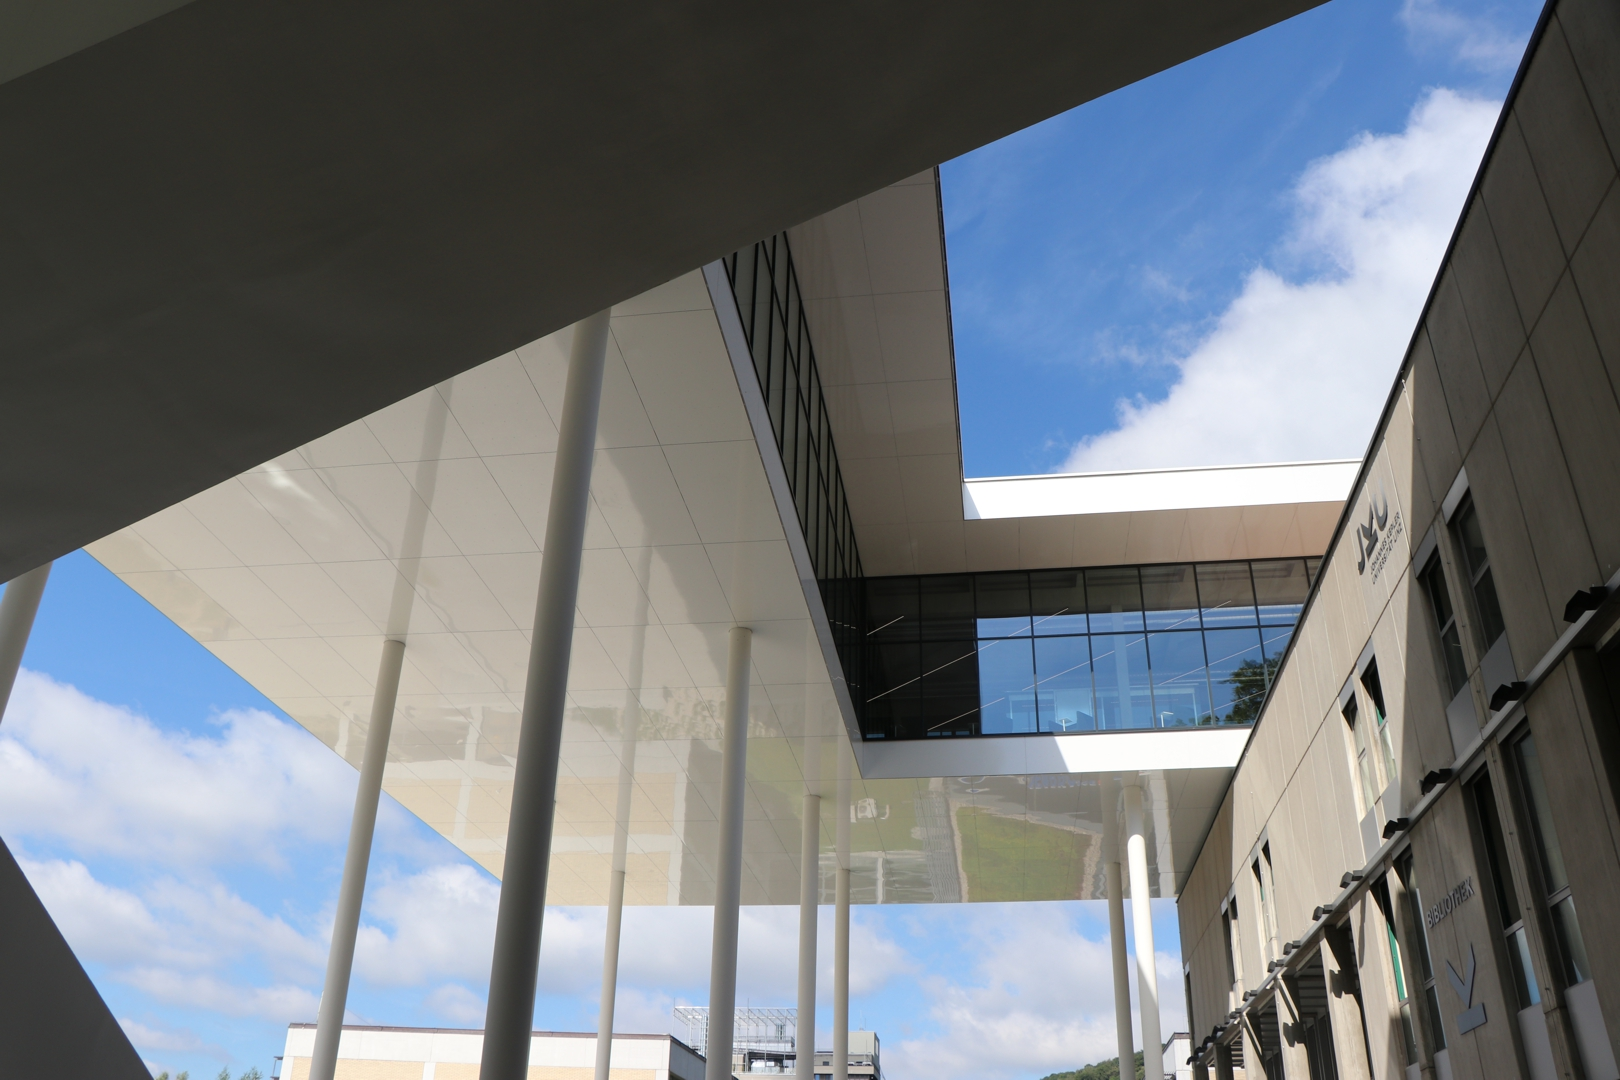
\includegraphics[width=\linewidth]{images/jku_learningcenter}
\caption{
    A figure. Be aware that figures have their caption below the artwork
}\label{fig:learningcenter}
\end{figure}
\begin{table}[t]
\centering
\caption{
    A table. Be aware that tables have their caption above the table
}\label{tab:nicetable}
\begin{tabularx}{\linewidth}{l>{\raggedright\arraybackslash}X}
\toprule
\textbf{Option}        & \textbf{Description} \\
\midrule
\texttt{phdthesis}     & PhD thesis \\
\texttt{mathesis}      & Master's thesis \\
\texttt{diplomathesis} & Diploma thesis \\
\texttt{bathesis}      & Bachelor's thesis \\
\texttt{seminarreport} & Seminar report \\
\texttt{techreport}    & Technical report \\
\bottomrule
\end{tabularx}
\end{table}

You will often reference and quote other works.
The source of these citations needs to be marked with the \string\cite\{\}\ command.
There are different ways to cite the work of others.
These are a few examples:
\begin{itemize}
\item The Tor directory authority moria1 shows a voting behavior for the HSDir flag that significantly deviates from that of other directory authorities~\cite{bib:2021-hoeller-iiwas}. Be aware that the \string\cite\ command is part of the sentence and, hence, comes before the period.
\item \citeauthor{bib:2015-roland-thesis-book}~\cite{bib:2015-roland-thesis-book} proposes a novel attack concept against NFC secure elements in mobile phones.
\item \citeauthor{bib:2013-roland-woot}~\cite{bib:2013-roland-woot} uncovered a flaw in legacy-support of the MasterCard contactless payment protocols that allows an attacker to clone certain credit cards.
\item \citeauthor{bib:2021-hoeller-foci}~\cite{bib:2021-hoeller-foci} designed an experiment to measure the usage of Tor V3 onion services in a privacy-conscious way. Here we used ``et al.'' because the cited work has more than two authors (\string\citeauthor\ will automatically take care of this).
\item \citeauthor{bib:2021-hoeller-iiwas}~\cite{bib:2021-hoeller-iiwas} conclude:
\begin{quote}
\emph{Ultimately, the high fluctuations in the hidden service directory were caused by a mixture of several issues. First the changed voting behavior of three directory authorities reduced the amount of obtainable votes to six. If any of the remaining six relays went offline -- which tends to happen during ongoing DOS attacks -- relays needed to obtain five out of five available votes. So any individual measurement failure regarding either bandwidth or uptime led to a withdrawn HSDir flag.}
\end{quote}
\item You sometimes also paraphrase from multiple sources. For that purpose, the \string\cite\ command accepts a list of multiple comma-separated references. Do not add spaces inbetween them. Various analyses of the Tor network have been performed recently~\cite{bib:2021-hoeller-foci,bib:2021-hoeller-iiwas}. 
\end{itemize}



\section{Conclusion}
\label{sec:conclusion}

Space for your summary, central conclusions, and an outlook on potential future work.


%% 
%%%%%%%%%%%%%%%%%%%%%%%%%%%%%%%%%%%%%%%%%%%%%%%%%%%%%%%%%%%%%%%%%%%%%%%%%%%%%%%%

%%%%%%%%%%%%%%%%%%%%%%%%%%%%%%%%%%%%%%%%%%%%%%%%%%%%%%%%%%%%%%%%%%%%%%%%%%%%%%%%
%% 
%% Print the bibliography
%% 
%% (Optionally) let the bibliography start on a new odd page (odd is only relevant in twoside layout)
%\cleardoubleoddpage
\printbibliography
%% 
%%%%%%%%%%%%%%%%%%%%%%%%%%%%%%%%%%%%%%%%%%%%%%%%%%%%%%%%%%%%%%%%%%%%%%%%%%%%%%%%

%% Begin with the appendix part (all further sections will be appendices)
\appendix

%%%%%%%%%%%%%%%%%%%%%%%%%%%%%%%%%%%%%%%%%%%%%%%%%%%%%%%%%%%%%%%%%%%%%%%%%%%%%%%%
%% 
%% Add your appendix sections ...
%% 

%% Make sure to start the appendix on a new odd page (odd is only relevant in twoside layout)
%\cleardoubleoddpage
\section{An Appendix}
\label{app:an-appendix}

Space for an appendix.
You can have more than one appendix section.
Appendices are, of course, optional.


%% 
%%%%%%%%%%%%%%%%%%%%%%%%%%%%%%%%%%%%%%%%%%%%%%%%%%%%%%%%%%%%%%%%%%%%%%%%%%%%%%%%

\cleardoubleoddpage

\end{document}
\endinput
